\begin{figure}[ht]
	\centering
	\subfloat[][Schemat cieplny]{
		\label{metody-teorii-grafow-przyklad.sch}
		\begin{tikzpicture}[thick]
			\node[boiler] (K) at (0,3.5) {K};
			\node[turbine] (T) at (5,4) {T};
			\node[condenser, font=\scriptsize] (S) at (5.75,2) {Sk};
			\node[pumpl, font=\scriptsize] (PS) at (4.5,.5) {PS};
			\node[heatxchg, font=\scriptsize] (R1) at (2.5,.5) {R1};

			{ [font=\scriptsize]
				\node[heatnode] (P0) at (0,5) {};
				\node[above] at (P0) {0};
				\node[heatnode] (P1) at (4.25,5) {};
				\node[above] at (P1) {1};
				\node[heatnode] (P2) at (5.75,3) {};
				\node[right] at (P2) {2};
				\node[heatnode] (P3) at (5.75,1) {};
				\node[left] at (P3) {3};
				\node[heatnode] (P4) at (3.75,.5) {};
				\node[above] at (P4) {4};
				\node[heatnode] (P5) at (1.5,.5) {};
				\node[above] at (P5) {5};
				\node[heatnode] (P6) at (4.25,3) {};
				\node[right] at (P6) {6};
				\node[heatnode] (P7) at (2.5,-.5) {};
				\node[left] at (P7) {7};
				\node[heatnode] (Pi) at (6.5,2.35) {};
				\node[above] at (Pi) {II};
				\node[heatnode] (Pii) at (6.5,1.65) {};
				\node[below] at (Pii) {I};
			}

			\draw (S.s) |- (PS.e);
			\draw (PS.w) -- (R1.e);
			\draw (R1.w) -| (K.s);

			{ [-stealth]
				\draw (K.n) |- (2,5) -| (T.nw);
				\draw (T.se) -- (S.n);

				\draw (T.sw) |- (3,3) -| (R1.n);
				\draw (R1.s) |- (6,-.5) -- ++(0,1.75) -- (S.s);
			}
		\end{tikzpicture}
	}

	\subfloat[][Wariant łukowy maszyn]{
		\label{metody-teorii-grafow-przyklad.w1}
		\begin{tikzpicture}
			{ [font=\scriptsize]
				\node[heatnode] (P0) at (1.5,5) {};
				\node[above] at (P0) {0};
				\node[heatnode] (P1) at (4.25,5) {};
				\node[above] at (P1) {1};
				\node[heatnode] (P2) at (5.75,3) {};
				\node[above] at (P2) {2};
				\node[heatnode] (P3k) at (5.75,.75) {};
				\node[heatnode] (P3) at (5,-.25) {};
				\node[above] at (P3) {3};
				\node[heatnode] (P4) at (2.75,.75) {};
				\node[left] at (P4) {4};
				\node[heatnode] (P5) at (2.75,3) {};
				\node[above] at (P5) {5};
				\node[heatnode] (P6) at (4.25,3) {};
				\node[above right] at (P6) {6};
				\node[heatnode] (P7) at (4.25,.75) {};
				\node[above right] at (P7) {7};
				\node[heatnode] (Pi) at (7.25,3) {};
				\node[above] at (Pi) {II};
				\node[heatnode] (Pii) at (7.25,.75) {};
				\node[below] at (Pii) {I};
			}

			{ [thick, -stealth, shorten >=1mm, shorten <=1mm, font=\scriptsize]
				\draw (P0) -- (P1) node[above, pos=.5] {(rurociąg)};
				\draw (P1) -- (P6);
				\draw (P6) -- (P2);
				\draw (P2) -- (P3k);
				\draw (P3k) -- (P3);
				\draw (P3) -| (P4) node[above right, pos=.4] {PS};
				\draw (P4) -- (P5);
				\draw (P5) -| (P0) node[above right, pos=.7, font=\small] {K};
				\draw (P6) -- (P7);
				\draw (P7) -- (P3);
				\draw (Pii) -- (Pi);
			}

			{ [color=red, dashdotted, font=\small, rounded corners]
				\draw (P6) +(-.1,-.1) rectangle (5.85,5.1);
				\path (P6) -- (5.85,5.1) node[pos=.5] {T};
				\draw (P4) +(-.1,-.1) rectangle (4.35,3.1);
				\draw (P3k) +(-.1,-.1) rectangle (7.35,3.1);
				\draw (P7) +(-.1,.1) rectangle (5.85,-.35);
				\path (P7) +(0,-.25) -- (P7 -| P3k)
					node[pos=.5, font=\scriptsize] {(miesz.)};
			}

			{ [color=blue, -stealth, shorten >=1mm, shorten <=1mm, font=\small]
				\path (P7) ++(0,.75) node (R1a) {};
				\path (P7) ++(0,1) node (R1b) {};
				\path (P7) ++(0,1.25) node (R1c) {};

				\draw (R1a.center) -- (R1a -| P5);
				\draw (R1b.center) -- (R1b -| P5);
				\draw (R1c.center) -- (R1c -| P5)
					node[above, pos=.5, color=red] {R1};

				\path (P3k) ++(0,.75) node (Ska) {};
				\path (P3k) ++(0,1) node (Skb) {};
				\path (P3k) ++(0,1.25) node (Skc) {};

				\draw (Ska.center) -- (Ska -| Pi);
				\draw (Skb.center) -- (Skb -| Pi);
				\draw (Skc.center) -- (Skc -| Pi)
					node[above, pos=.5, color=red] {Sk};
			}
		\end{tikzpicture}
	}%
	~ %
	\subfloat[][Wariant węzłowy maszyn]{
		\label{metody-teorii-grafow-przyklad.w2}
		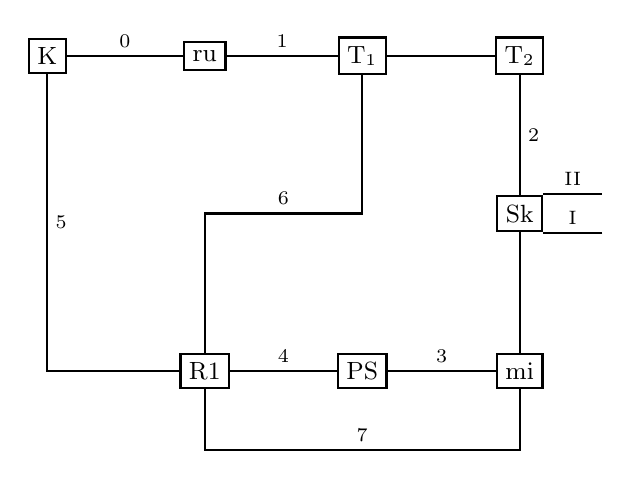
\begin{tikzpicture}[thick]
			{ [rectangle, font=\small, minimum size=8mm]
				\node[draw] (K) at (0,4) {K};
				\node[draw] (ru) at (2,4) {ru};
				\node[draw] (T1) at (4,4) {T$_1$};
				\node[draw] (T2) at (6,4) {T$_2$};
				\node[draw] (S) at (6,2) {Sk};
				\node[draw] (mi) at (6,0) {mi};
				\node[draw] (PS) at (4,0) {PS};
				\node[draw] (R1) at (2,0) {R1};
			}

			{ [-stealth, font=\scriptsize]
				\draw (K.east) -- (ru.west) node[above, pos=.5] {0};
				\draw (ru.east) -- (T1.west) node[above, pos=.5] {1};
				\draw (T1.east) -- (T2.west);
				\draw (T2.south) -- (S.north) node[right, pos=.5] {2};
				\draw (S.south) -- (mi.north);
				\draw (mi.west) -- (PS.east) node[above, pos=.5] {3};
				\draw (PS.west) -- (R1.east) node[above, pos=.5] {4};
				\draw (R1.west) -| (K.south) node[right, pos=.75] {5};

				\draw (T1.south) |- (4,2) -| (R1.north) node[above, pos=.25] {6};
				\draw (R1.south) |- (4,-1) -| (mi.south) node[above, pos=0] {7};

				{ [blue]
					\draw (S.east) ++(0,.25) -- ++(.75,0) node[above, pos=.5] {II};
					\draw (S.east) ++(.75,-.25) -- ++(-.75,0) node[above, pos=.5] {I};
				}
			}
		\end{tikzpicture}
	}

	\caption{Reprezentacja przykładowego obiegu cieplnego za~pomocą teorii grafów}
	\label{metody-teorii-grafow-przyklad}
\end{figure}
